\documentclass{beamer}\usepackage[]{graphicx}\usepackage[]{color}
%% maxwidth is the original width if it is less than linewidth
%% otherwise use linewidth (to make sure the graphics do not exceed the margin)
\makeatletter
\def\maxwidth{ %
  \ifdim\Gin@nat@width>\linewidth
    \linewidth
  \else
    \Gin@nat@width
  \fi
}
\makeatother

\definecolor{fgcolor}{rgb}{0.345, 0.345, 0.345}
\newcommand{\hlnum}[1]{\textcolor[rgb]{0.686,0.059,0.569}{#1}}%
\newcommand{\hlstr}[1]{\textcolor[rgb]{0.192,0.494,0.8}{#1}}%
\newcommand{\hlcom}[1]{\textcolor[rgb]{0.678,0.584,0.686}{\textit{#1}}}%
\newcommand{\hlopt}[1]{\textcolor[rgb]{0,0,0}{#1}}%
\newcommand{\hlstd}[1]{\textcolor[rgb]{0.345,0.345,0.345}{#1}}%
\newcommand{\hlkwa}[1]{\textcolor[rgb]{0.161,0.373,0.58}{\textbf{#1}}}%
\newcommand{\hlkwb}[1]{\textcolor[rgb]{0.69,0.353,0.396}{#1}}%
\newcommand{\hlkwc}[1]{\textcolor[rgb]{0.333,0.667,0.333}{#1}}%
\newcommand{\hlkwd}[1]{\textcolor[rgb]{0.737,0.353,0.396}{\textbf{#1}}}%
\let\hlipl\hlkwb

\usepackage{framed}
\makeatletter
\newenvironment{kframe}{%
 \def\at@end@of@kframe{}%
 \ifinner\ifhmode%
  \def\at@end@of@kframe{\end{minipage}}%
  \begin{minipage}{\columnwidth}%
 \fi\fi%
 \def\FrameCommand##1{\hskip\@totalleftmargin \hskip-\fboxsep
 \colorbox{shadecolor}{##1}\hskip-\fboxsep
     % There is no \\@totalrightmargin, so:
     \hskip-\linewidth \hskip-\@totalleftmargin \hskip\columnwidth}%
 \MakeFramed {\advance\hsize-\width
   \@totalleftmargin\z@ \linewidth\hsize
   \@setminipage}}%
 {\par\unskip\endMakeFramed%
 \at@end@of@kframe}
\makeatother

\definecolor{shadecolor}{rgb}{.97, .97, .97}
\definecolor{messagecolor}{rgb}{0, 0, 0}
\definecolor{warningcolor}{rgb}{1, 0, 1}
\definecolor{errorcolor}{rgb}{1, 0, 0}
\newenvironment{knitrout}{}{} % an empty environment to be redefined in TeX

\usepackage{alltt}
\usetheme{metropolis}           % Use metropolis theme
\usepackage{amsmath}
\usepackage{amssymb}
\usepackage{float}
\usepackage{listings}
\usepackage{graphicx}
\usepackage{subfigure}
\usepackage{tikz}
\usetikzlibrary{shapes.geometric, arrows}
\usetikzlibrary{shapes.geometric, arrows}
\tikzset{
  int/.style={circle, draw=black, fill=blue!20, minimum size=3em},
  int2/.style={circle, draw=black, fill=red!20, minimum size=3em},
  int3/.style={circle, draw=black, fill=green!20, minimum size=3em},
  init/.style={pin distance=1.2cm,pin edge={loop,thin,black}}
}
\tikzstyle{arrow} = [thick,black,->,>=stealth]
\tikzstyle{pinstyleto} = [pin edge={<-,thick,black}]
\tikzstyle{pinstyleout} = [pin edge={->,thick,black}]



%\titlegraphic{\centering \includegraphics[height=2cm, width=7cm]{titlepic.pdf}\vfill }
\titlegraphic{\centering \includegraphics[height=10cm, width=20cm]{images/titlepic.pdf} }
\title{Spatial Epidemics Dynamics: Synchronization}
\subtitle{Mathematics 4MB3/6MB3\\Mathematical Biology}
\date{\today}
\author{Model Students: Nicole Dumont, Melody Fong, Carolina Weishaar}
%\institute{Centre for Modern Beamer Themes}
\IfFileExists{upquote.sty}{\usepackage{upquote}}{}
\begin{document}
  \maketitle
  
\begin{frame}{Table of Contents}
  \setbeamertemplate{section in toc}[sections numbered]
  \tableofcontents[hideallsubsections]
\end{frame}

  \section{Introduction}
  \begin{frame}{Diseases are fun}
    Text goes here
  \end{frame}
  \begin{frame}{Diseases are cool}
    Text goes here
  \end{frame}
  
  \section{Methods}
    \begin{frame}{Forced SIR Model for a Single Patch}
  \begin{center}
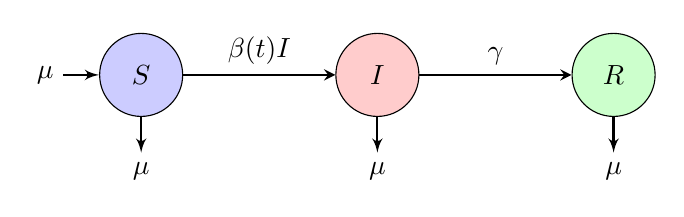
\begin{tikzpicture}[node distance=3cm,auto,>=latex',every node/.append style={align=center}]
    \node [int, pin={[pinstyleto]left:$\mu$}, pin={[pinstyleout]below:$\mu$}] (a)              {$S$};
    \node [int2, pin={[pinstyleout]below:$\mu$}] (b) [right of=a] {$I$};
    \node [int3, pin={[pinstyleout]below:$\mu$}] (c) [right of=b] {$R$};
    
    \draw [arrow] (a) -- node[anchor=south] {$ \beta(t) I $} (b);
    \draw [arrow] (b) -- node[anchor=south] {$\gamma$} (c);
\end{tikzpicture}
\begin{align*}
  \frac{dS}{dt} &= \mu -\beta(t) S I -\mu S \\ 
  \frac{dI}{dt} &= \beta(t) S I -\gamma I - \mu I \\
  \frac{dR}{dt} &= \gamma I -\mu R
\end{align*}

\begin{align*}
  \beta(t) &= \left < \beta \right > (1+\alpha \cos(2\pi t)) \\
  \left < \beta \right > &= \mathcal{R}_0 (\mu + \gamma)
\end{align*}
\end{center}
   \end{frame}
  
  \begin{frame}{Metapatch SIR Model}
  \begin{center}
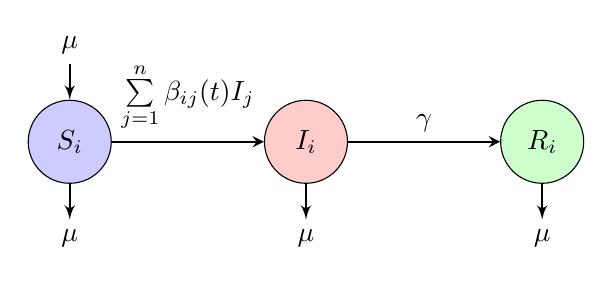
\begin{tikzpicture}[node distance=3cm,auto,>=latex',every node/.append style={align=center}]
    \node [int, pin={[pinstyleto]above:$\mu$}, pin={[pinstyleout]below:$\mu$}] (a)   {$S_i$};
    \node [int2, pin={[pinstyleout]below:$\mu$}] (b) [right of=a] {$I_i$};
    \node [int3, pin={[pinstyleout]below:$\mu$}] (c) [right of=b] {$R_i$};
    
    \draw [arrow] (a) -- node[anchor=south] {$ \sum\limits_{j=1}^{n}\beta_{ij}(t) I_j $} (b);
    \draw [arrow] (b) -- node[anchor=south] {$\gamma$} (c);
\end{tikzpicture}
\begin{align*}
  \frac{dS_i}{dt} &= \mu - S_i\sum\limits_{j=1}^{n}\beta_{ij}(t) I_j -\mu S_i \\ 
  \frac{dI_i}{dt} &= S_i\sum\limits_{j=1}^{n}\beta_{ij}(t) I_j -\gamma I_i - \mu I_i \\
  \frac{dR_i}{dt} &= \gamma I_i -\mu R_i
\end{align*}
\end{center}
   \end{frame}
   
   \begin{frame}{Beta Matrix}
    \begin{equation*}
  \beta(t) = \left < \beta \right > (1+\alpha \cos(2\pi t))M
\end{equation*}

Equal Coupling Matrix:
  \[
M =
\begin{bmatrix}
  1-m & \frac{m}{n-1} & \frac{m}{n-1} & \frac{m}{n-1} & \dots \\
  \frac{m}{n-1} & 1-m & \frac{m}{n-1} & \frac{m}{n-1}  \\
  \frac{m}{n-1} & \frac{m}{n-1} & 1-m &  \\
  \vdots &  &  & \ddots 
\end{bmatrix}
\]

  \end{frame}
  
  \begin{frame}{Beta Matrix}
    \begin{equation*}
  \beta(t) = \left < \beta \right > (1+\alpha \cos(2\pi t))M
\end{equation*}
Nearest Neighbour Matrix:
  \[
M =
\begin{bmatrix}
  1-m & \frac{m}{2} & 0 & 0 & \dots & \frac{m}{2} \\
  \frac{m}{2} & 1-m & \frac{m}{2} & 0 & & \vdots \\
  0 & \frac{m}{2} & 1-m &  \\
  0 & 0 & & \ddots \\
  \vdots & & & & \ddots & \frac{m}{2} \\
  \frac{m}{2} &  & & \dots & \frac{m}{2} & 1-m \ 
\end{bmatrix}
\]
  \end{frame}
  
  \section{Results}
  
  \begin{frame}{Bifurcation Diagram}
   Single Patch SIR model with sinusoidal seasonal forcing
   \centering 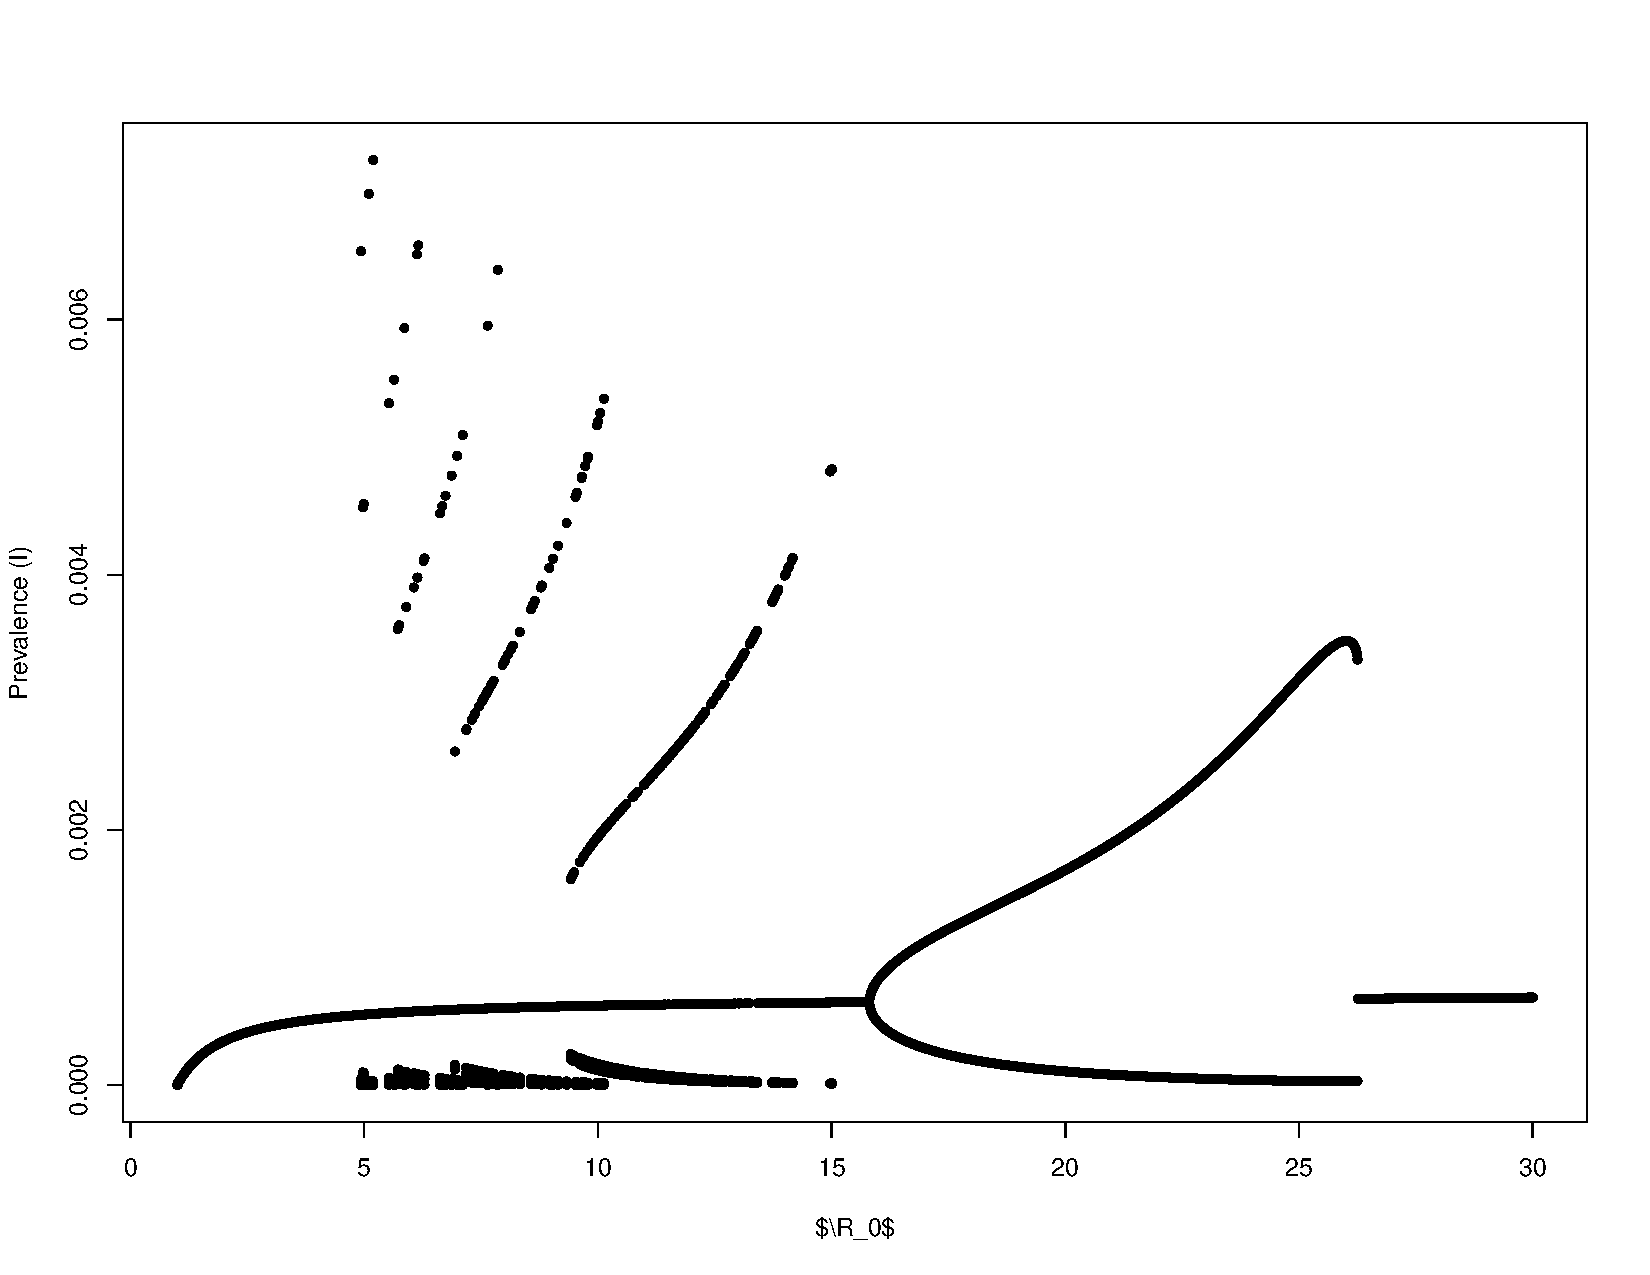
\includegraphics[width=0.7\linewidth]{{images/bifurcation}.pdf}
   \end{frame}
   
   \begin{frame}{Period Diagram}
   Period of the oscillations
   \centering 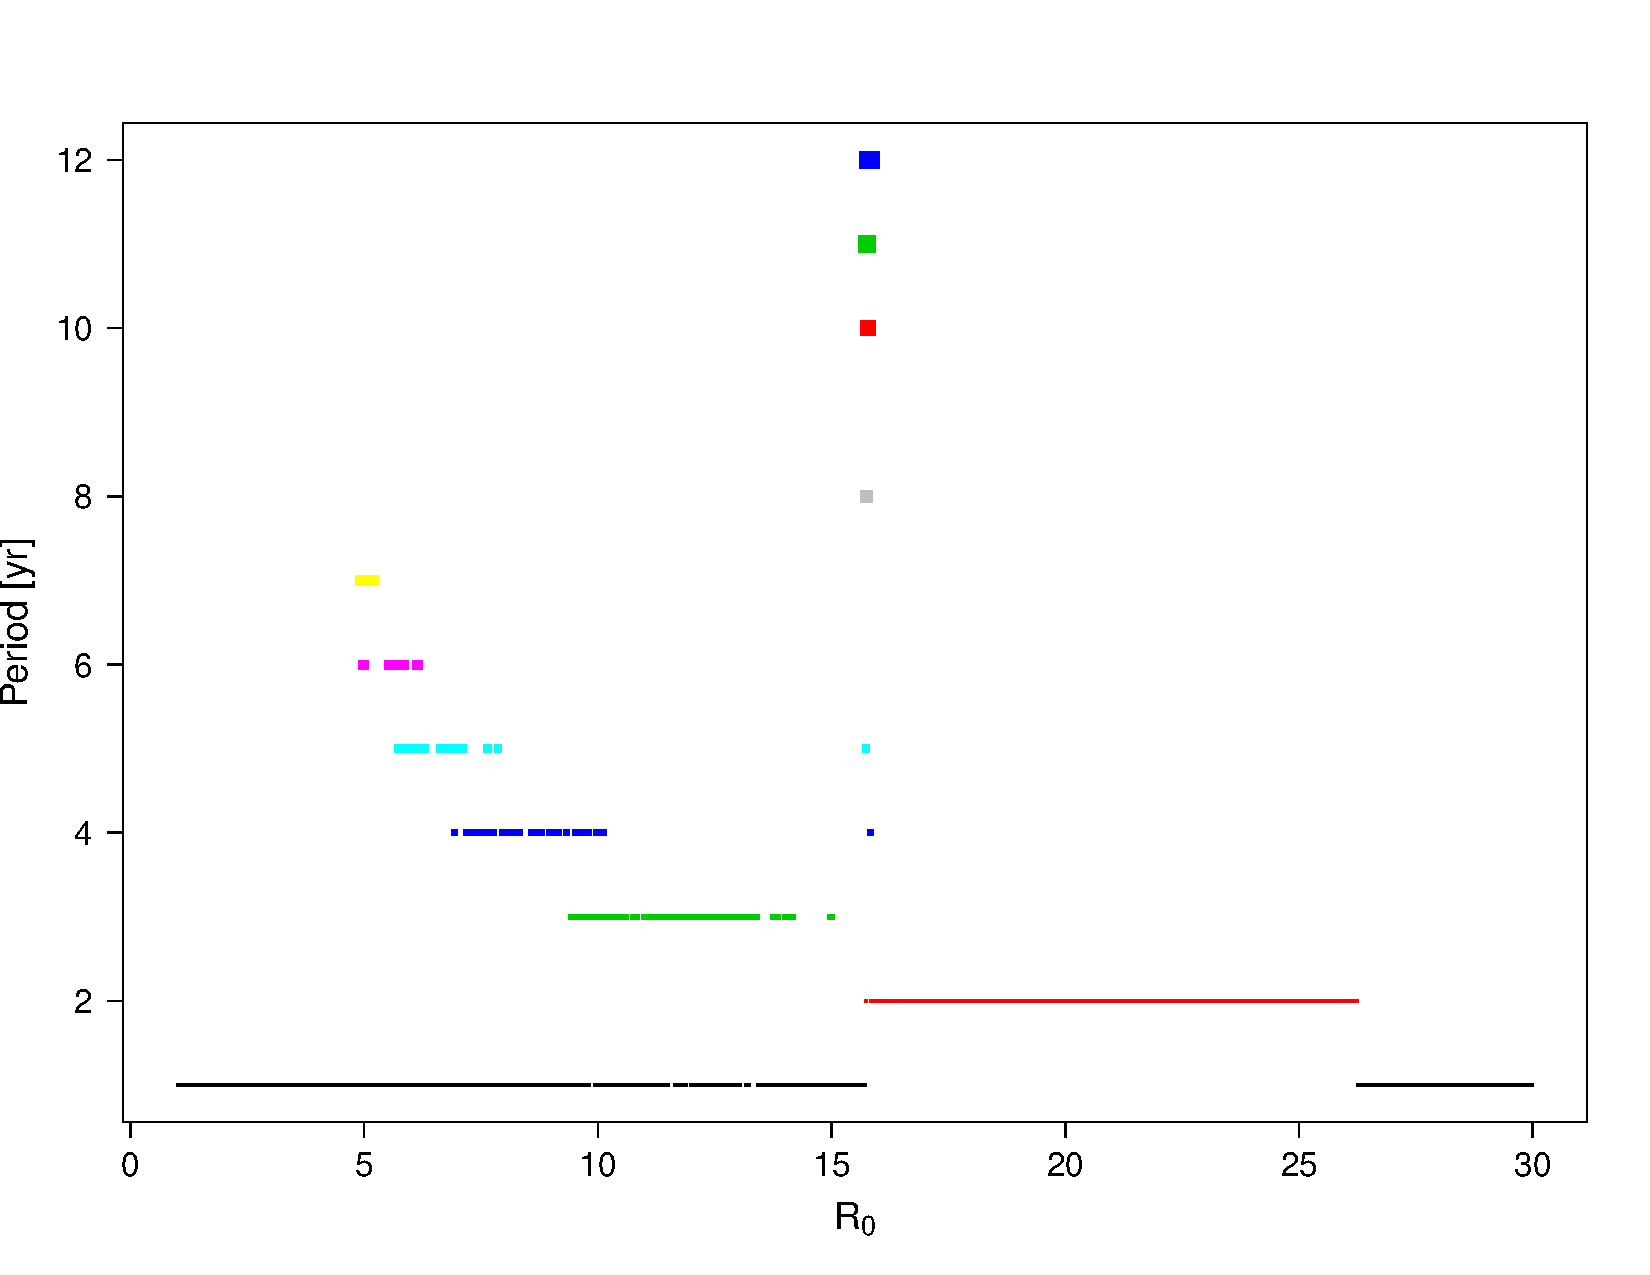
\includegraphics[width=0.7\linewidth]{{images/period}.pdf}
   \end{frame}

   \begin{frame}{Deterministic Model}
   Nearest Neighbour Coupling, $\mathcal{R}_0=17$, $m=0.2$
   \centering 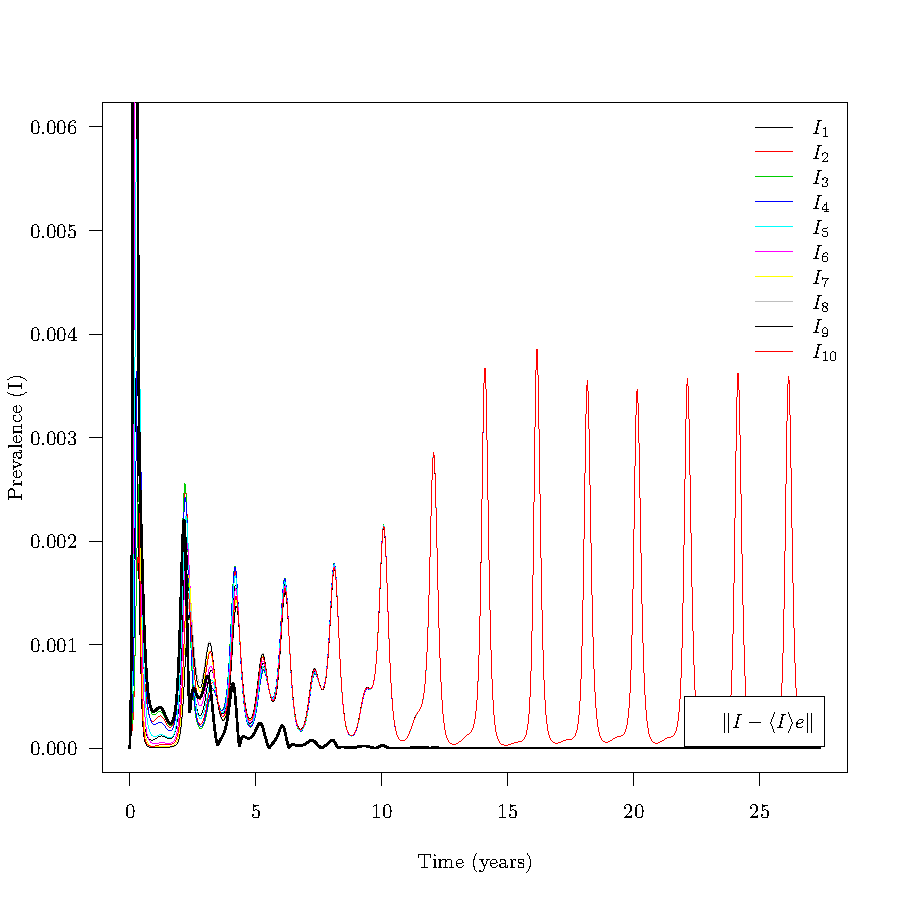
\includegraphics[width=0.7\linewidth]{{images/detNNR017m0.2}.pdf}
   \end{frame}
   
   \begin{frame}{Deterministic Model}
   Equal Coupling, $\mathcal{R}_0=17$, $m=0.2$
   \centering 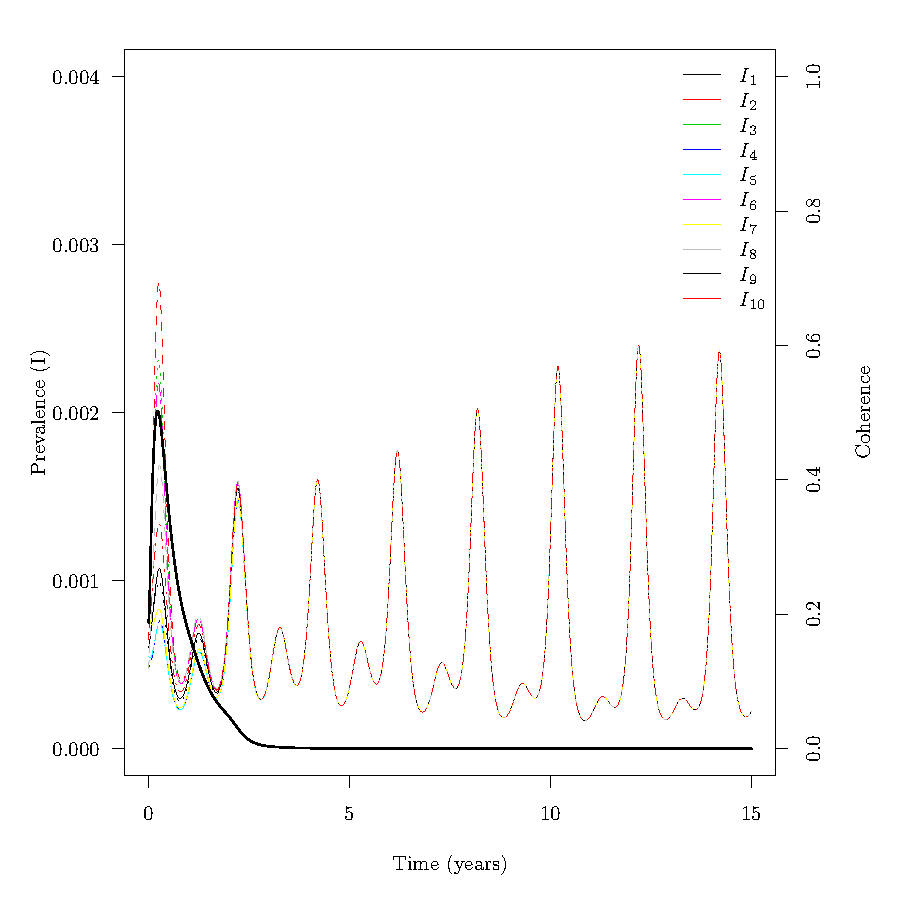
\includegraphics[width=0.7\linewidth]{{images/detECR017m0.2}.pdf}
   \end{frame}
   
   \begin{frame}{Deterministic Model}
   Nearest Neighbour Coupling, $\mathcal{R}_0=17$, $m=0.01$
   \centering 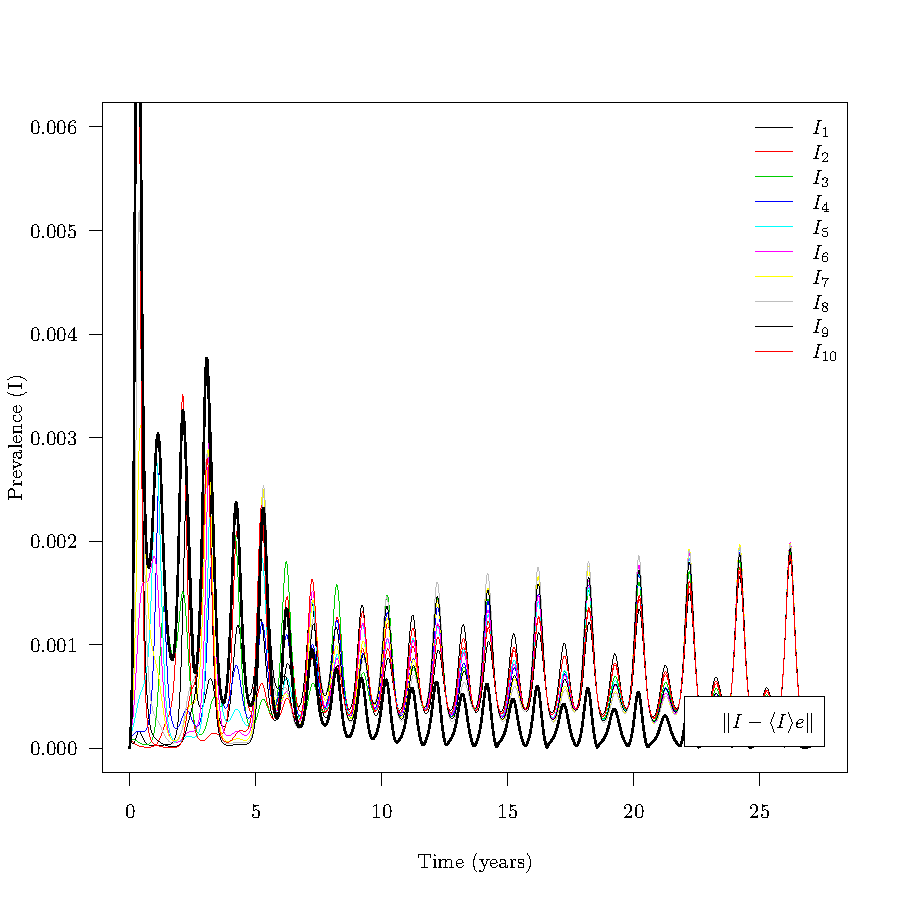
\includegraphics[width=0.7\linewidth]{{images/detNNR017m0.01}.pdf}
   \end{frame}
   
   \begin{frame}{Deterministic Model}
   \begin{centering}
   Nearest Neighbour Coupling, $m=0.2$
     \begin{columns}
      \begin{column}{0.5\textwidth}
      \scalebox{0.8}{\parbox{.5\linewidth}{%
       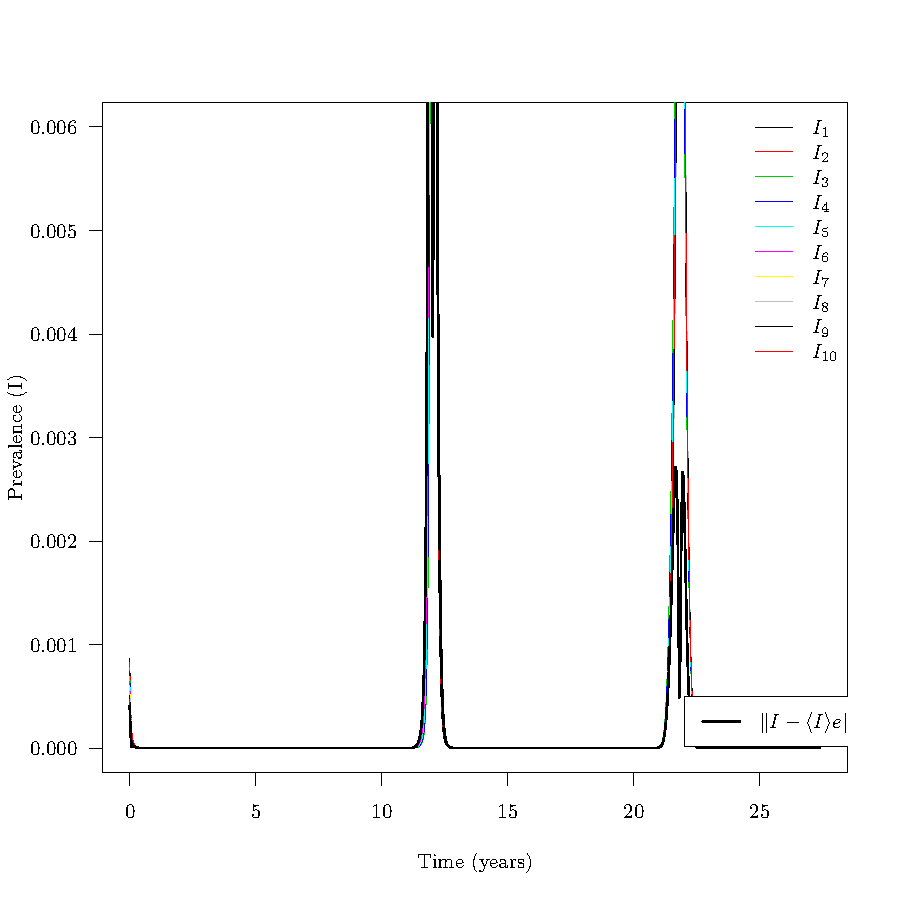
\includegraphics[width=2.2\linewidth]{{images/detNNR06m0.2}.pdf} \\
      $\mathcal{R}_0=6$
      }}
     \end{column}
    \begin{column}{0.5\textwidth}
    \scalebox{0.8}{\parbox{.5\linewidth}{%
       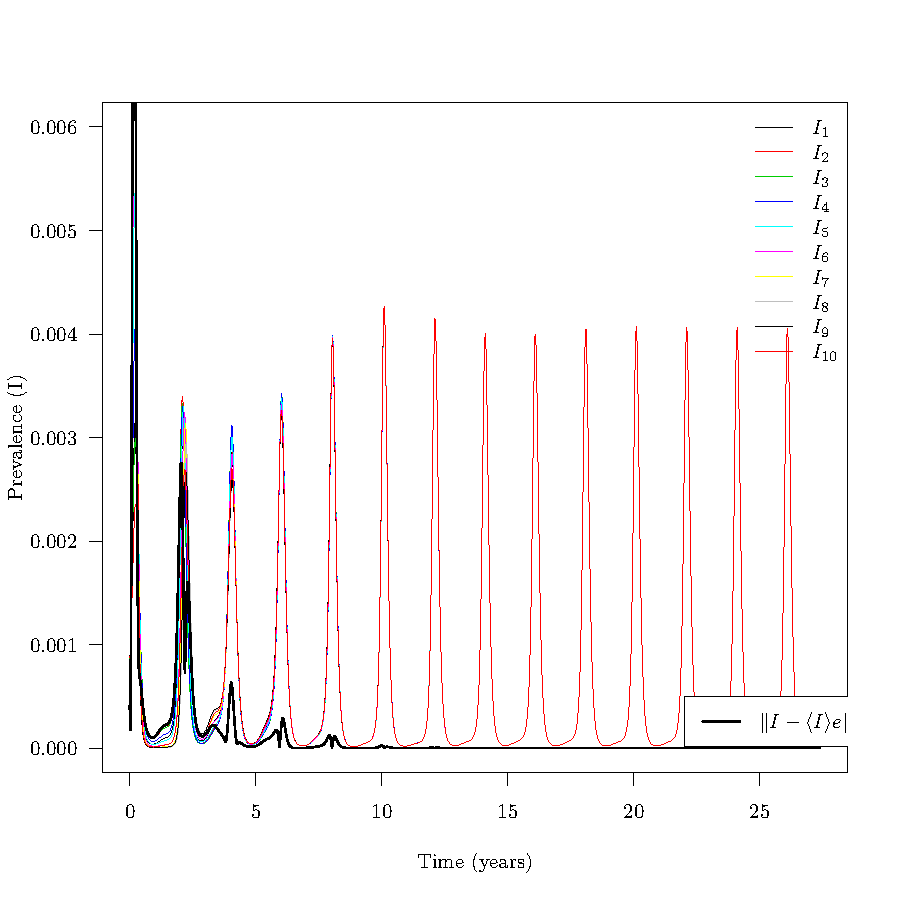
\includegraphics[width=2.2\linewidth]{{images/detNNR025m0.2}.pdf} \\
       $\mathcal{R}_0=25$
      }}
    \end{column}
    \end{columns}
    \end{centering}
   \end{frame}
   
   \begin{frame}{Stochastic: Gillespie Model}
   Equal Coupling, Population of 3000, $\mathcal{R}_0=17$, $m=0.2$
   \centering 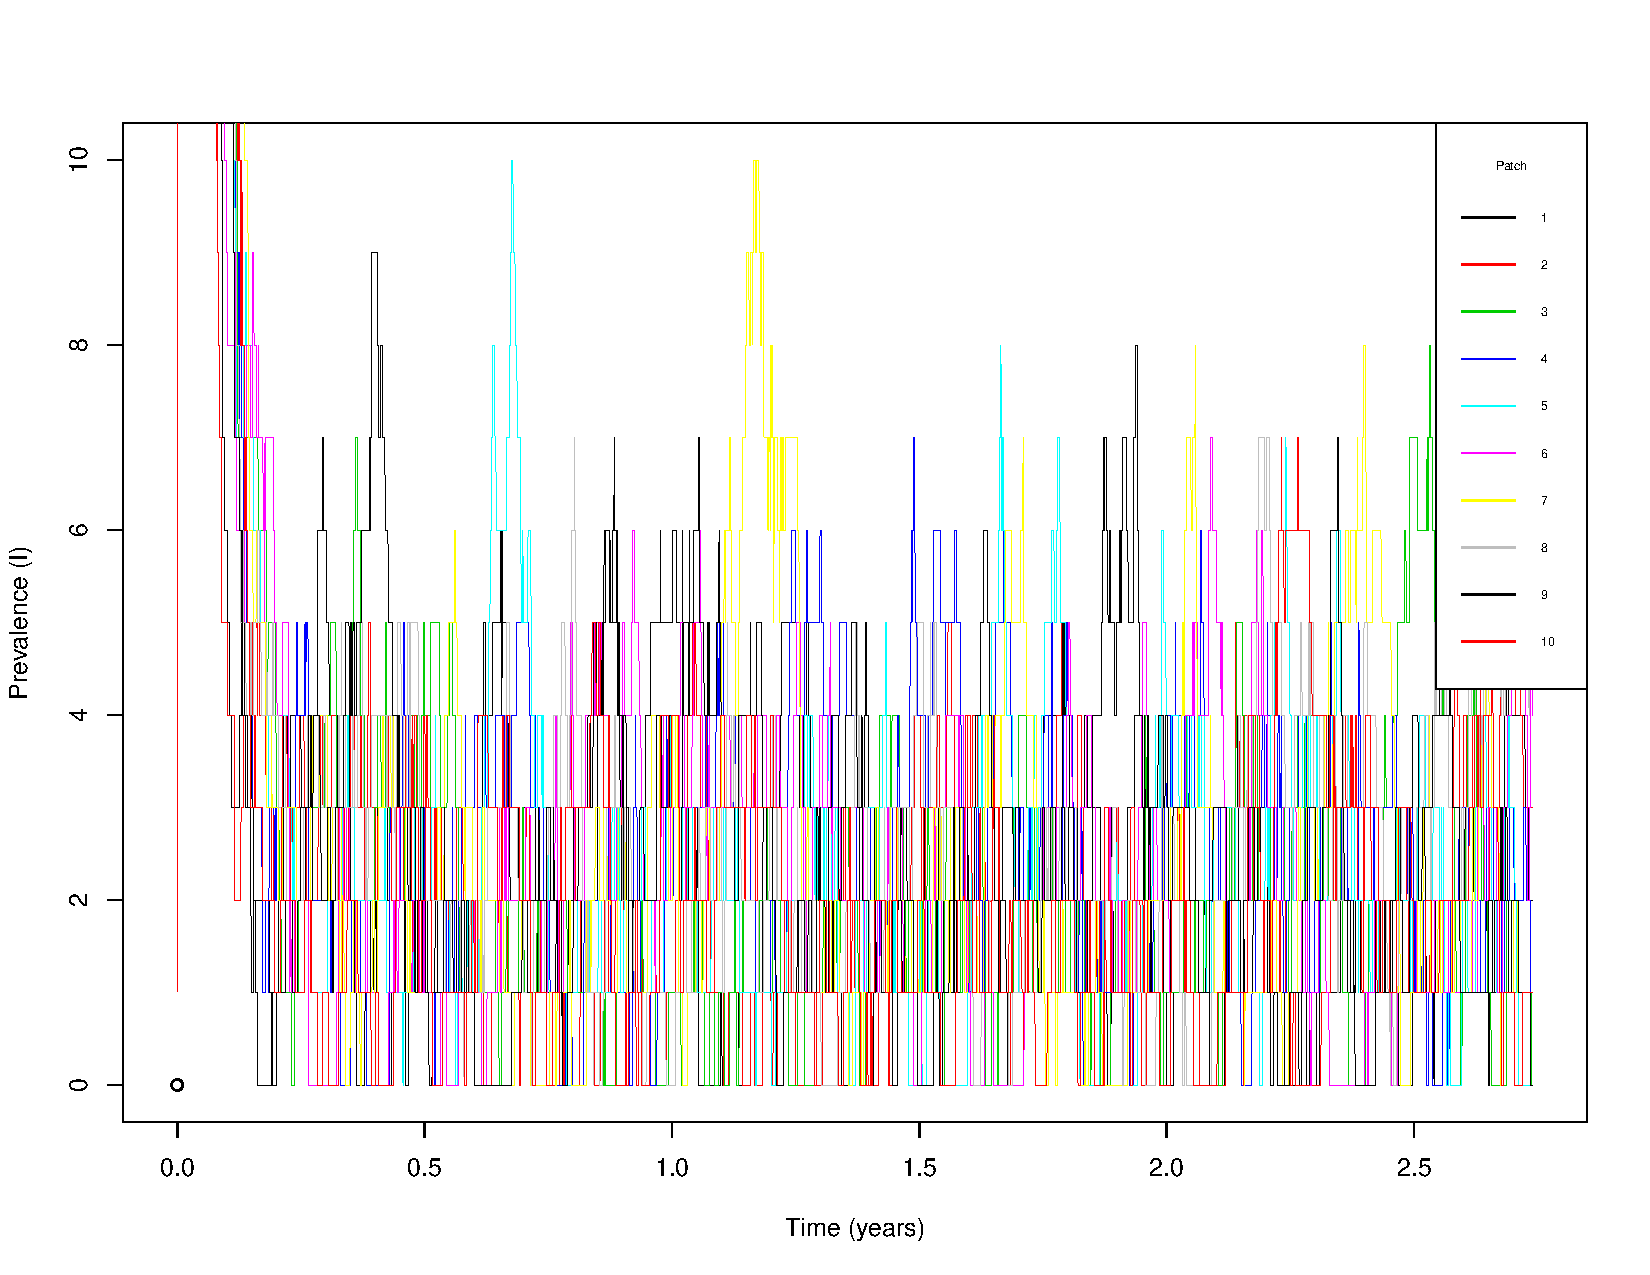
\includegraphics[width=0.7\linewidth]{{images/GillECR017m0.2small}.pdf}
   \end{frame}
   
   \begin{frame}{Stochastic: Gillespie Model}
   Equal Coupling, Population of , $\mathcal{R}_0=17$, $m=0.2$
   \centering 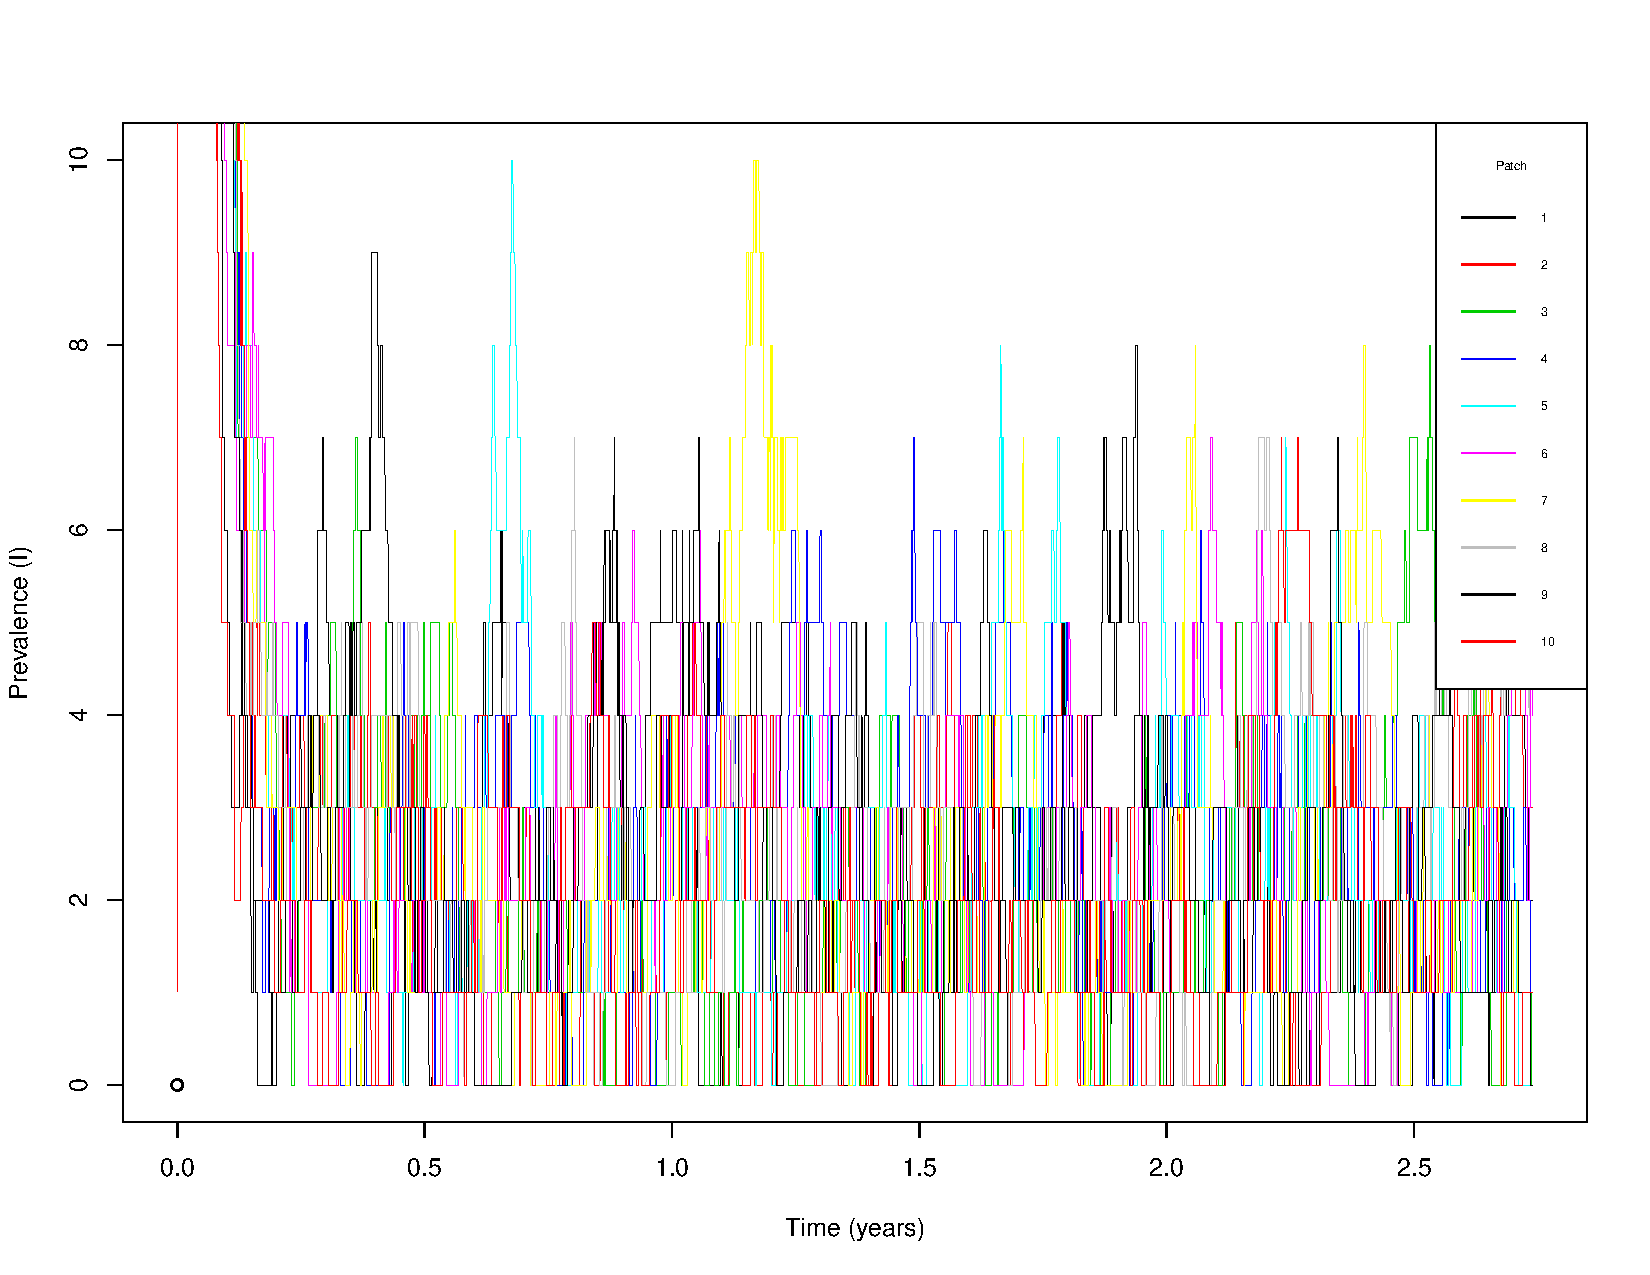
\includegraphics[width=0.7\linewidth]{{images/GillECR017m0.2}.pdf}
   \end{frame}
   
   \begin{frame}{Stochastic: Adaptive Tau Algorthim}
   Equal Coupling, Population of 500000, $\mathcal{R}_0=18.69$, $m=0.2$
   \centering 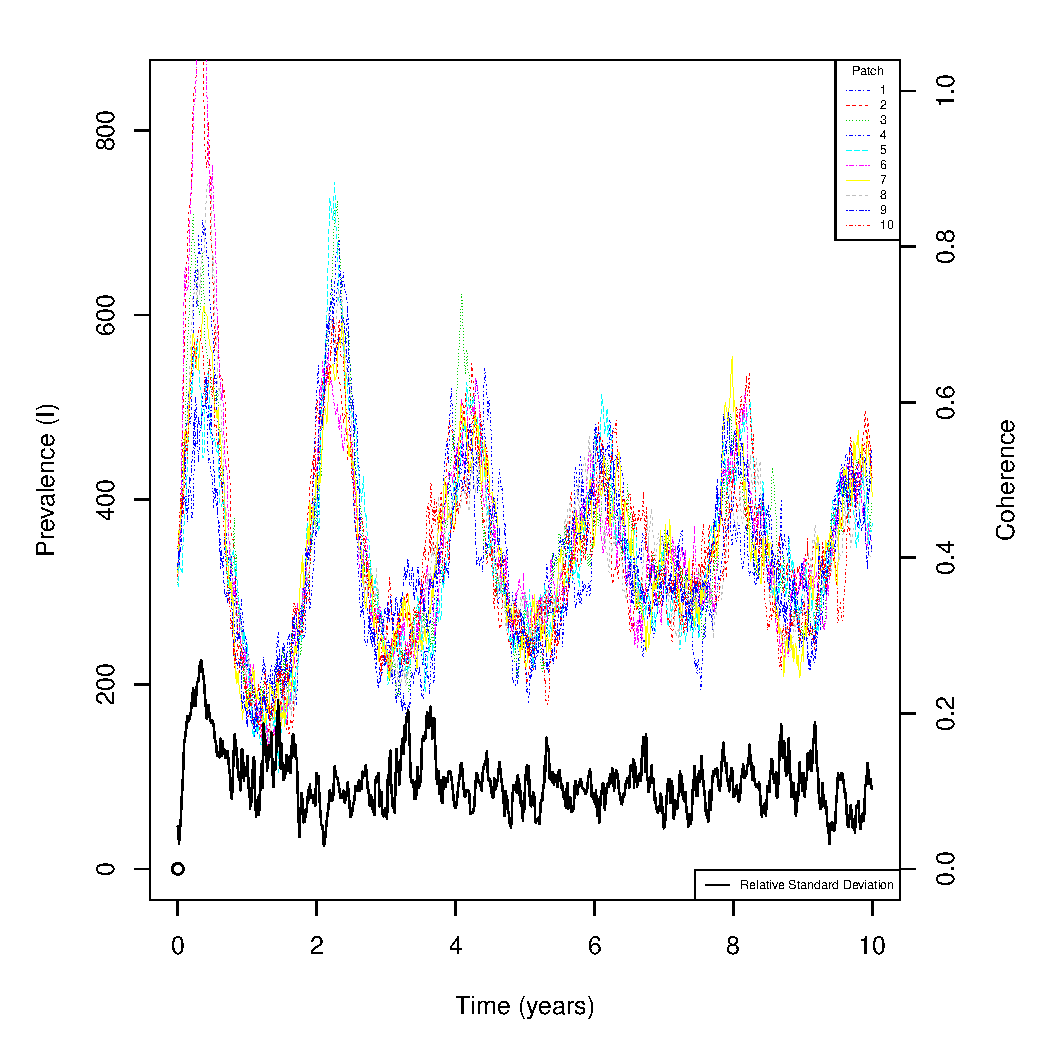
\includegraphics[width=0.7\linewidth]{{images/adaptauECR018.6869m0.2}.pdf}
   \end{frame}
   
   \begin{frame}{Coherence dependence on Parameters}
   \end{frame}
   
\begin{frame}[standout]
  Questions?
\end{frame}

\appendix


\begin{frame}[allowframebreaks]{References}

  \bibliography{demo}
  \bibliographystyle{abbrv}

\end{frame}
   
\end{document}
